%* 
%* ------------------------------------------------------------------
%* TTTutorial.tex - Time Table (V2) Tutorial
%* Created by Robert Heller on Thu Apr 26 12:32:29 2007
%* ------------------------------------------------------------------
%* Modification History: $Log$
%* Modification History: Revision 1.1  2007/05/06 12:49:40  heller
%* Modification History: Lock down  for 2.1.8 release candidate 1
%* Modification History:
%* Modification History: Revision 1.1  2002/07/28 14:03:50  heller
%* Modification History: Add it copyright notice headers
%* Modification History:
%* ------------------------------------------------------------------
%* Contents:
%* ------------------------------------------------------------------
%*  
%*     Model RR System, Version 2
%*     Copyright (C) 1994,1995,2002-2005  Robert Heller D/B/A Deepwoods Software
%* 			51 Locke Hill Road
%* 			Wendell, MA 01379-9728
%* 
%*     This program is free software; you can redistribute it and/or modify
%*     it under the terms of the GNU General Public License as published by
%*     the Free Software Foundation; either version 2 of the License, or
%*     (at your option) any later version.
%* 
%*     This program is distributed in the hope that it will be useful,
%*     but WITHOUT ANY WARRANTY; without even the implied warranty of
%*     MERCHANTABILITY or FITNESS FOR A PARTICULAR PURPOSE.  See the
%*     GNU General Public License for more details.
%* 
%*     You should have received a copy of the GNU General Public License
%*     along with this program; if not, write to the Free Software
%*     Foundation, Inc., 675 Mass Ave, Cambridge, MA 02139, USA.
%* 
%*  
%* 

\chapter{Time Table (V2) Tutorial}
\label{chpt:tt:Tutorial}
\typeout{$Id$}

\index{Time Table!Tutorial|(} The Time Table is a program designed to
create railroad employee timetables.  The program's main display is a
graph of time (of day) versus distance (along the railroad), gridded at
time intervals and at station stops.  Trains schedules are represented
as colored lines on this graph, with diagonals representing train
movement at speed and horizontal lines representing trains ``siting''
at stations (layovers or switching).

\section{Creating a new time table}

To create an new time table select the \verb=File->New= menu item or
the 
\includegraphics{TTNewTool.png} toolbar button. A ``Create a New
Time Table'' dialog, described in
Section~\ref{sect:tt:createnewtimetable}. is displayed.  This dialog
box collects three pieces of information: the name of the new time
table, the total time (in minutes) the time table will cover (there are
1440 minutes in a 24 hour day), and the tick interval in minutes.  A
new time table can also me created from the command line by including
the options \verb=-totaltime= and \verb=-timeincrement= along with a
name for the new time table.

\subsection{Creating stations}

Once the name and the two time elements have been selected, a set of at
least two stations need to be created.  This is done with the ``Create
All Stations Dialog'',  described in
Section~\ref{sect:tt:CreateAllStationsDialog}.  This dialog box is
used to create stations, which can have zero or more storage tracks. 
Storage tracks are used when a train has a long layover (and needs to
be ``out of the way'' of other traffic) or when a train terminates and
the train set is re-used for a different schedule, generally in the
opposite direction. As the stations and their storage tracks are
created, they are displayed in the station listing in the upper part of
the dialog. 

\subsection{Creating cabs}

After creating all of the stations, zero or more cabs can be created. 
Cabs are mostly for switched block DC layouts, but creating ``cabs''
for a DCC layout is useful, since it allows for a way to visually group
trains operationally. Think of the cabs as a way of defining ``crews''
(operators).  This allows for things like crew (operator) changes as
the train moves to different parts of the layout for example.

\section{Creating trains}

Once the stations and cabs have been created, the program displays an
empty chart.  The chart's \verb=x= axis is time (in minutes).  The upper
section of the chart has the cabs (if any), the middle part of the chart
has the stations, and the bottom part of the chart has the storage
tracks (if any).  Now we can create a train.  This is done by selecting
either the \verb=Trains->Add Train= menu item, clicking on the add train
(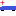
\includegraphics{TTaddtrain.png}) toolbar button or the 
\verb=Add a new train= button.  All of these display the ``Create New
Train Dialog'', described in Section~\ref{sect:tt:CreateNewTrainDialog}.

Trains have a (common) name, a number (or symbol), a class number, an average
speed, a scheduled departure time, and travel between two stations.  The
train's number (or symbol) needs to be a unique identification of the
train. The class is a whole number, with smaller numbers generally being
the ``higher'' class.  The class is used to indicate a train's priority
and is also used to group similar trains together.  The speed is the
(scale) speed the train will be traveling between stops.  The scheduled
departure time is the time the train is scheduled to leave its origin
station.  The origin and termination stations are the station end points
the train travels between.  The train will get a ``stop'' at every
intermediate station between these two stations.  Note that the train
won't be expected to actually stop at any station where the layover time
is set to zero.  Such stops would just be timekeeping points.

Once the train's basic information is set, the \verb=Schedule= button can be
clicked.  This shifts to the schedule page, where layovers and cab
assignments cab be set.  The \verb=Update= buttons propagate the
cab settings and adjust the times to allow for the layovers.  If the
train makes use of station storage tracks, the \verb=Storage= button can
be clicked and storage tracks selected.  When the train is fully
configured, the \verb=Done= button can be clicked to actually create the
train.

\section{Printing a time table}

Once all of the trains have been added, it it possible to ``print'' a
timetable.  The LaTeX system is used to format the time table and the
TimeTable program generates a \LaTeX{} source file (\verb=.tex=) and will
run the \LaTeX{} program, \verb=pdflatex=, to create a PDF file from the
\LaTeX{} source file.  This process is started with the
\verb=File->Print...= menu item or the
\includegraphics{TTprintTool.png} toolbar button.  This pops up the
``Print Dialog'', described in Section~\ref{sect:tt:PrintTimetableDialog}.
This dialog collects the name of the \LaTeX{} source file, and the path to the
\LaTeX{} processing programing, as well as a few other options.  It also
has a button to configure how the timetable will be formatted.  

The \verb=Configure= button pops up the ``Print Configuration Dialog'',
described in Section~\ref{sect:tt:PrintConfigurationDialog}, which has
three sections, a \verb=General= section which gets some general
configuration settings, a \verb=Multi= section for various
configuration settings relating to printing multiple tables, and a
\verb=Groups= section, for configuring groups of trains.  Some of the
configuration assumes some knowledge of \LaTeX. A visit to the \TeX{} and
\LaTeX{} web pages (\url{http://www.tug.org}) is a good place to start,
with the beginner's page at \url{http://www.tug.org/begin.html} as the
obvious starting point.  You don't really have to learn how to use
\LaTeX{}, you just need to have a \TeX/\LaTeX{} system installed.  The only
other issue is the \verb=TimeTable.sty= file.  This file either needs to be
installed somewhere in the \TeX/\LaTeX{} search path or it needs to be in
the same directory as the \LaTeX{} source file generated by the TimeTable
program. You will need to learn a little about \LaTeX{} if you want to
include various sorts of customizations.
\index{Time Table!Tutorial|)} 
